\documentclass{article}
\usepackage{graphicx}
\usepackage[margin=1.5cm]{geometry}
\usepackage{amsmath}

\begin{document}

\title{Wednesday Reading Assessment: Unit 1 and kinematics}
\author{Prof. Jordan C. Hanson}

\maketitle

\section{Memory Bank}

\begin{align}
v(t) &= \frac{dx}{dt} \\
a(t) &= \frac{dv}{dt}
\end{align}

\section{Chapter 3.2}

\begin{figure}[ht]
\centering
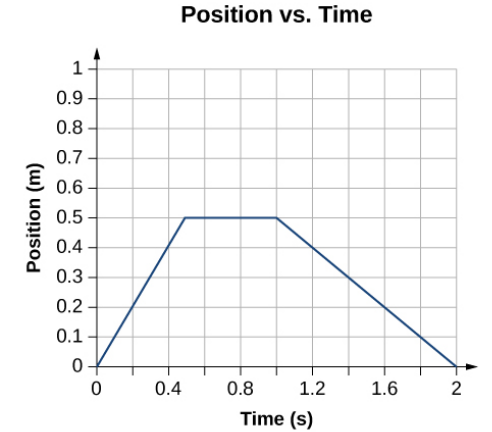
\includegraphics[width=0.3\textwidth]{figures/x_vs_t.png}
\caption{\label{fig:graph} A graph of the displacement versus time of a system, in meters versus seconds.}
\end{figure}

\begin{enumerate}
\item Consider Fig. \ref{fig:graph}.  (a) What is the velocity implied by the line segment between 0 and 0.5 seconds? (b) What is the velocity implied by the line segment between 0.5 and 1.0 seconds? (c) What is the velocity implied by the line segment between 1.0 and 2.0 seconds? \\ \vspace{1cm}
\item Write an formula that describes the 3rd line segment, and call this $v(t)$.  What is the acceleration or deceleration? \\ \vspace{2cm}
\item Draw an example curve on Fig. \ref{fig:graph} that implies negative acceleration.
\end{enumerate}

\end{document}
